\section{Background}

\subsection{Tensor Contractions}
\label{sec:tensorContractions}

%TODO: HOW THE HELL DO I INTRODUCE MATH?!
Tensor contractions are a generalization of batched matrix multiplications on n-dimensional arrays called order-n tensors.
In a binary contraction of two tensors $A$ and $B$ to a third tensor $C$ we will refer to the first input tensor $A$ as left tensor and the second input tensor $B$ as the right one. %todo: will hier in Ordnung?
We use the following classification for the dimensions in the tensors $A$,$B$ and $C$:

\begin{tabular}{ |c|c|c|c| } 
  \hline
  $dimension type$ & present in A & present in B & present in C\\
  \hline
  $c$ & $\checkmark$& $\checkmark$& $\checkmark$\\
  $m$ & $\checkmark$& $\crossmark$& $\checkmark$\\
  $n$ & $\crossmark$& $\checkmark$& $\checkmark$\\
  $k$ & $\checkmark$& $\checkmark$& $\crossmark$\\
  \hline
 \end{tabular}



\subsection{Einsum expressions}

Einsum expressions allow for a more succinct expression than the typical Tensor notation as used in \ref{sec:tensorContractions}.
Instead of writing $C_{pstuv}=\sum_{q}\sum_{r}A_{pqrs}B_{tuqvr}$ the same contraction is expressed as $A_{pqrs}B_{tuqvr} \rightarrow C_{pstuv}$.
The summation signs are now implicit.
Einsum expressions can also describe the contractions of more than 2 tensors\cite{einsum_is_all_you_need}.
%todo: can I just recommend people to look at resources such as "Einsum is all you need" for an advanced introduction?
Instead of writing $D_{ij} = \sum_{k}\sum_{l}A_{ik}B_{jkl}C_{il}$ it is expressed as $A_{ik}B_{jkl}C_{il} \rightarrow D_{ij}$.
All expression in the rest of this thesis are written as simplified einsum expression, either written as $A,B\rightarrow C$, leaving out the indices, or as $pqrs,tuqvr \rightarrow pstuv$, leaving out the tensor variables.
The evaluation of einsum expression is supported in the popular frameworks Torch\cite{torch}, PyTorch\cite{pytorch} and Tensorflow\cite{tensorflow}.

\subsection{einsum\_ir}
\label{sec:einsum_ir}

\begin{figure}[ht]
  \centering{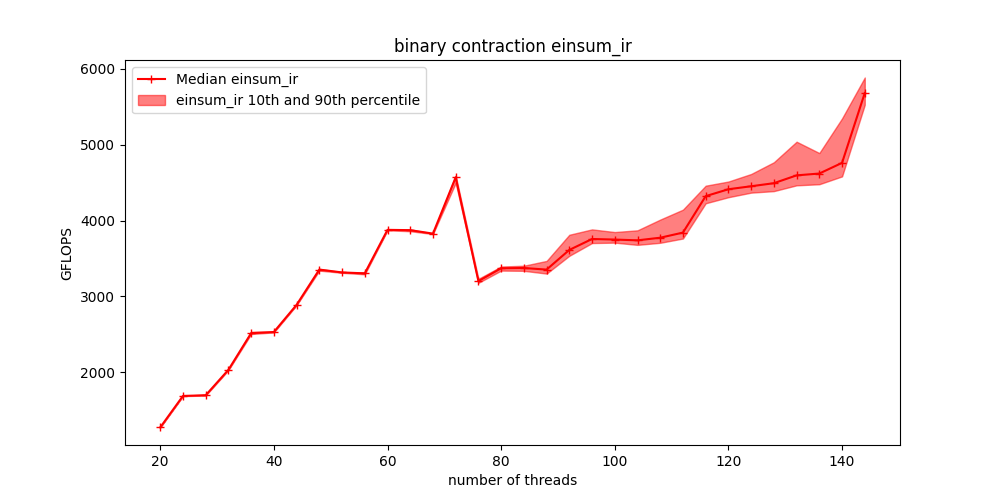
\includegraphics[width=0.95\textwidth]{gflops_threads.png}}
  \caption{
    Performance of einsum\_ir on an Nvidia Grace CPU Superchip.
    Grace consists of 2 72-core CPUs connected via NVLink.
    The contraction used is $m_0c_0k_0k_1m_1, n_0c_0k_0n_0n_1 \rightarrow m_0n_0c_0n_1m_1$ with $|c_0|=2$, $|m_0|=|n_0|=|k_0|$ and $|m_1|=|n_1|=|k_1|=70$.
  }
  \label{fig:perf_threads}
\end{figure}

\texttt{einsum\_ir}\cite{einsum_ir} is a software to evaluate a series of einsum expressions expressed in tree form.
An example for an einsum tree is $[A,B\rightarrow C],D \rightarrow E$.
My work builds on top of this software, using their implementation of a binary tensor contraction $A,B \rightarrow C$ as local primitive for my algorithm.
\texttt{einsum\_ir} already implements shared memory parallelization with OpenMP\cite{openMP}, so it can already exploit all CPU cores on a single NUMA domain.
Its performance is currently not scaling well across more than one CPU, as seen in Figure \ref{fig:perf_threads}.
The performance drops as soon as the threads of the second CPU get used, as seen in the sharp decline after 72 threads and Grace.
This thesis provides algorithms for a secondary distributed memory parallelization to improve scaling across CPUs.
An important note for the current binary tensor contraction interface is that it expects all tensors, both input and output, to be stored in contiguous memory.
